% vim:encoding=utf8 ft=tex sts=2 sw=2 et:

\documentclass{classrep}
\usepackage[utf8]{inputenc}

\usepackage{listings}
\usepackage{graphicx}
\studycycle{Informatyka, studia niestacjonarne}
\coursesemester{IV}

%\coursename{Angelologia teoretyczna i stosowana}
\coursename{Inteligentna Analiza Danych}
\courseyear{2017/2018}

\courseteacher{mgr Rogalski}
\coursegroup{sobota, 10:30}

\author{
  \studentinfo{Marcin Pajkowski}{211968} \and
  \studentinfo{Rafał Warda}{214067}
}

\title{Zadanie 2b: Klasyfikacja}

\begin{document}
\maketitle

\section{Wstęp}
Celem zadania było wykorzystanie wcześniej napisanego programu implementującego koncepcję perceptronu wielowarstwowego do klasyfikacji zestawu "Iris Flower Data Set".

\section{Opis realizacji zadania}
\subsection{Odwzorowanie tekstowej reprezentacji danych}
Zestaw irysów składa się z 150 rekordów. W każdym wierszu pierwsze cztery wartości numeryczne opisują atrybuty kwiatu - kolejno długość i szerokość działki kielicha oraz długość i szerokość płatka. Wartości te są wyrażone w centymetrach. Piątym polem jest etykieta klasy:

- Iris-setosa,

- Iris-versicolor,

- Iris-virginica.
\newline
Aby etykiety klas przekształcić na wartość liczbową (i tym samym przystosować format danych do zgodnego z specyfiką projektu) wprowadzono wyjścia, które będą kolejno reprezentować stuprocentowe prawdopodobieństwo przynależności do danej klasy (oraz dla dwóch pozostałych - prawdopodobieństwo równe 0\%). Zgodnie z przyjętą nomenklaturą predykowane wyjście dla klasy "setosa" to 1 0 0, dla klasy "versicolor" 0 1 0. a dla klasy "virginica" 0 0 1. Odpowiednio spreprawowany plik tekstowy jest podawany do aplikacji.
\subsection{Podział zbioru}
Zbiór 150 irysów został podzielony na dwa podzbiory: podzbiór danych treningowych oraz podzbiór danych testowych. Podział został dokonany w proporcji 2:1 - spośród 150 rekordów co trzeci "wpada" do puli danych testowych.
\subsection{Część badawcza}
\subsubsection{Opis części badawczej}
W tym badaniu zostaną zaprezentowane możliwości aplikacji w znacznie szerszym zakresie niż miało to miejsce w zadaniu poprzednim. Manipulatory takie jak współczynnik momentum, współczynnik nauki czy obecność biasu pozostaną nietknięte i przyjmą wartości:

-momentum: 0.9

-nauka: 0.2

-bias: aktywny
\newline
Zmieniana będzie natomiast sama konfiguracja sieci w sensie ilości warstw ukrytych oraz ilości neuronów na każdej z nich
\subsubsection{Konfiguracja 4,3,3}
Wykres nauki w czasie (próbkowanie co 20 epok)
\begin{center}
 \includegraphics{output_0_0.pdf}
 % output_0_1.pdf: 382x252 px, 72dpi, 13.48x8.89 cm, bb=0 0 382 252
\end{center}
Błąd średniokwadratowy zestawu testowego: 0,0.000830
\newpage
\subsubsection{Konfiguracja 4,4,3}
Wykres nauki w czasie (próbkowanie co 20 epok)
\begin{center}
 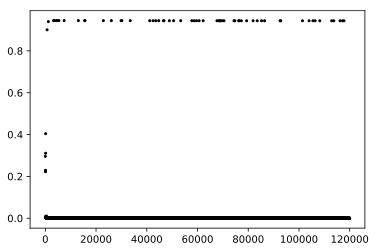
\includegraphics{output_0_1.pdf}
 % output_0_1.pdf: 382x252 px, 72dpi, 13.48x8.89 cm, bb=0 0 382 252
\end{center}
Błąd średniokwadratowy zestawu testowego: 0,0.000830
\subsubsection{Konfiguracja 4,3,4,3}
Wykres nauki w czasie (próbkowanie co 20 epok)
\begin{center}
 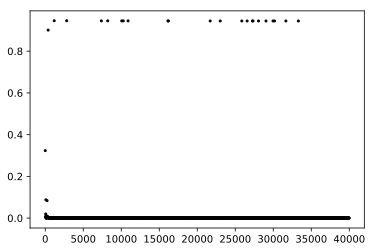
\includegraphics{output_0_2.pdf}
 % output_0_1.pdf: 382x252 px, 72dpi, 13.48x8.89 cm, bb=0 0 382 252
\end{center}
Błąd średniokwadratowy zestawu testowego: 0,0.000828
\newpage
\subsubsection{Konfiguracja 4,7,3}
Wykres nauki w czasie (próbkowanie co 20 epok)
\begin{center}
Wykres nauki w czasie (próbkowanie co 20 epok)
 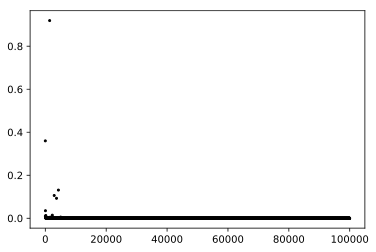
\includegraphics{output_0_3.pdf}
 % output_0_1.pdf: 382x252 px, 72dpi, 13.48x8.89 cm, bb=0 0 382 252
\end{center}
\subsubsection{Konfiguracja 4,4,3,3}
\begin{center}
Wykres nauki w czasie (próbkowanie co 20 epok)
 \includegraphics{output_0_4.pdf}
 % output_0_1.pdf: 382x252 px, 72dpi, 13.48x8.89 cm, bb=0 0 382 252
\end{center}
Błąd średniokwadratowy zestawu testowego: 0,0.000002
%\begin{thebibliography}{0}
  %\bibitem{l2short} T. Oetiker, H. Partl, I. Hyna, E. Schlegl.
   % \textsl{Nie za krótkie wprowadzenie do systemu \LaTeX2e}, 2007, dostępny
    %online.
%\end{thebibliography}
\end{document}
